% !TeX root = ./2020-21-COMP250-04-session-materials_screen.tex
% Adjust these for the path of the theme and its graphics, relative to this file
%\usepackage{beamerthemeFalmouthGamesAcademy}
\usepackage[T1]{fontenc}
\usepackage{../../beamerthemeFalmouthGamesAcademy}
\usepackage{multimedia}
\graphicspath{ {../../} }

% Default language for code listings
\lstset{language=C++,
        morekeywords={each,in,nullptr}
}

% For strikethrough effect
\usepackage[normalem]{ulem}
\usepackage{wasysym}

\usepackage{pdfpages}

\usepackage{algpseudocode}

% http://www.texample.net/tikz/examples/state-machine/
\usetikzlibrary{arrows,automata}

\usepackage{pgfplots}
\pgfplotsset{width=\textwidth,height=0.6\textheight,compat=1.9}

\newcommand{\modulecode}{COMP260}\newcommand{\moduletitle}{Distributed Systems}\newcommand{\sessionnumber}{5}

\begin{document}
\title{\sessionnumber: Utility-Based AI}
\subtitle{\modulecode: \moduletitle}

\frame{\titlepage} 

% !TeX root = ./2020-21-COMP250-04-session-materials_screen.tex
\part{Utility}
\frame{\partpage}

\renewcommand{\pounds}{\text{\textsterling}}

\begin{frame}{Utility theory}
    \begin{itemize}
        \pause\item How does an AI agent measure ``goodness'' or ``usefulness'' of the outcomes of its actions?
        \pause\item \textbf{Utility theory} supposes that a given outcome can be assigned a \textbf{single number} 
            measuring its \textbf{utility}
        \pause\item Actions can then be \textbf{ranked} by utility, and one with the \textbf{highest} utility chosen
        \pause\item Utility is sometimes called \textbf{reward}, \textbf{payoff}, \textbf{fitness}
        \pause\item Multiply by $-1$ and we have \textbf{cost}
    \end{itemize}
\end{frame}

\begin{frame}{Utility --- example}
    \begin{itemize}
        \pause\item A laptop costs $\pounds 500$ from Amazon or $\pounds 450$ from Bob's Computers
        \pause\item Assuming everything else equal, where do you buy it from?
    \end{itemize}
\end{frame}

\begin{frame}{Utility --- example}
    \begin{itemize}
        \pause\item A laptop costs $\pounds 500$ from Amazon or $\pounds 450$ from Bob's Computers
        \pause\item Amazon offers next-day delivery, but delivery from Bob's Computers takes 4 weeks
        \pause\item Assuming everything else equal, where do you buy it from?
        \pause\item Utility is a \textbf{single number} ---
            we essentially have to put a monetary value on the longer wait time
    \end{itemize}
\end{frame}

\begin{frame}[fragile]{Weighting}
    \begin{itemize}
        \pause\item Utility is often formed of several \textbf{decision factors}
        \pause\item In the laptop buying example: price and delivery time
        \pause\item To get a utility value we can take a \textbf{weighted sum}
        \begin{lstlisting}
utility = WEIGHT_PRICE * price + WEIGHT_TIME * time;
        \end{lstlisting}
        \pause\item Here \lstinline{WEIGHT_PRICE} and \lstinline{WEIGHT_TIME} are constant values
        \pause\item The values used will influence the agent's behaviour and so must be carefully tuned by the designer
    \end{itemize}
\end{frame}

\begin{frame}{Nonlinearity}
    \begin{itemize}
        \pause\item Decision factors are not always linear
        \pause\item E.g.\ a difference of $\pounds 1$ is more significant for something that costs $\pounds 5$
            than something that costs $\pounds 500$
        \pause\item E.g.\ a difference of 1 HP is more significant if the agent is close to death
            than if it is at full health
        \pause\item Therefore we may want to apply a \textbf{curve} mapping to decision factors 
    \end{itemize}
\end{frame}

\begin{frame}[fragile]{Polynomial curve}
    \begin{columns}
        \begin{column}{0.57\textwidth}
            \begin{center}
                \begin{tikzpicture}
                    \begin{axis}[
                            axis lines = left,
                            xlabel = $x$,
                            ylabel = {$y=x^3$},
                        ]
                        \addplot [
                            domain=0:1, 
                            samples=100, 
                        ]
                        {x^3};
                    \end{axis}
                \end{tikzpicture}
            \end{center}
        \end{column}
        \begin{column}{0.4\textwidth}
            \begin{itemize}
                \pause\item Formula: $y = x^k$
                \pause\item C\#: \lstinline{Mathf.Pow(x, k)}
                \pause\item $k$ is a constant: bigger $k$ gives a steeper curve
            \end{itemize}
        \end{column}
    \end{columns}
\end{frame}

\begin{frame}{Inverse polynomial curve}
    \begin{columns}
        \begin{column}{0.57\textwidth}
            \begin{center}
                \begin{tikzpicture}
                    \begin{axis}[
                            axis lines = left,
                            xlabel = $x$,
                            ylabel = {$y=x^{1/3}$},
                        ]
                        \addplot [
                            domain=0:1, 
                            samples=100, 
                        ]
                        {x^0.333333};
                    \end{axis}
                \end{tikzpicture}
            \end{center}
        \end{column}
        \begin{column}{0.4\textwidth}
            \begin{itemize}
                \pause\item Same formula as polynomial curve, but $k$ is between 0 and 1
                \pause\item $k$ closer to $0$ gives a steeper curve
            \end{itemize}
        \end{column}
    \end{columns}
\end{frame}

\begin{frame}[fragile]{Step function}
    \begin{columns}
        \begin{column}{0.57\textwidth}
            \begin{center}
                \begin{tikzpicture}
                    \begin{axis}[
                            axis lines = left,
                            xlabel = $x$,
                            ylabel = {$y$},
                        ]
                        \addplot [
                            domain=0:1
                        ]
                        coordinates {(0,0) (0.5,0) (0.5,1) (1,1)};
                    \end{axis}
                \end{tikzpicture}
            \end{center}
        \end{column}
        \begin{column}{0.4\textwidth}
            \begin{itemize}
                \pause\item Formula: $y = \begin{cases}
                    0 &\text{if } x<0.5 \\
                    1 &\text{if } x \geq 0.5
                \end{cases}$
                \pause\item C\#: \lstinline{(x < 0.5f) ? 0 : 1}
                \pause\item Models a \textbf{threshold} or \textbf{if-then} rule
            \end{itemize}
        \end{column}
    \end{columns}
\end{frame}

\begin{frame}[fragile]{Logistic function}
    \begin{columns}
        \begin{column}{0.5\textwidth}
            \begin{center}
                \begin{tikzpicture}
                    \begin{axis}[
                            axis lines = left,
                            xlabel = $x$,
                            ylabel = {$y=\frac{1}{1+e^{-10x}}$},
                        ]
                        \addplot [
                            domain=-1:1, 
                            samples=100, 
                        ]
                        {1 / (1 + exp(-10*x))};
                    \end{axis}
                \end{tikzpicture}
            \end{center}
        \end{column}
        \begin{column}{0.47\textwidth}
            \begin{itemize}
                \pause\item Formula: $y = \frac{1}{1+e^{-kx}}$
                \pause\item C\#: \lstinline{1 / (1 + Mathf.Exp(-k*x))}
                \pause\item Similar to step function but with a softer transition from ``off'' to ``on''
                \pause\item $k$ is a constant: bigger $k$ gives a steeper curve
            \end{itemize}
        \end{column}
    \end{columns}
\end{frame}

\begin{frame}{Tweaking curves}
    \begin{itemize}
        \pause\item Adjusting utility curves is \textbf{more art than science}
        \pause\item It's worth \textbf{experimenting} with different curve types to get the desired result
        \pause\item \textbf{Graphical curve editors} are worth investigating
        \pause\item E.g.\ InstinctAI asset for Unity:
    \end{itemize}
    \begin{center}
        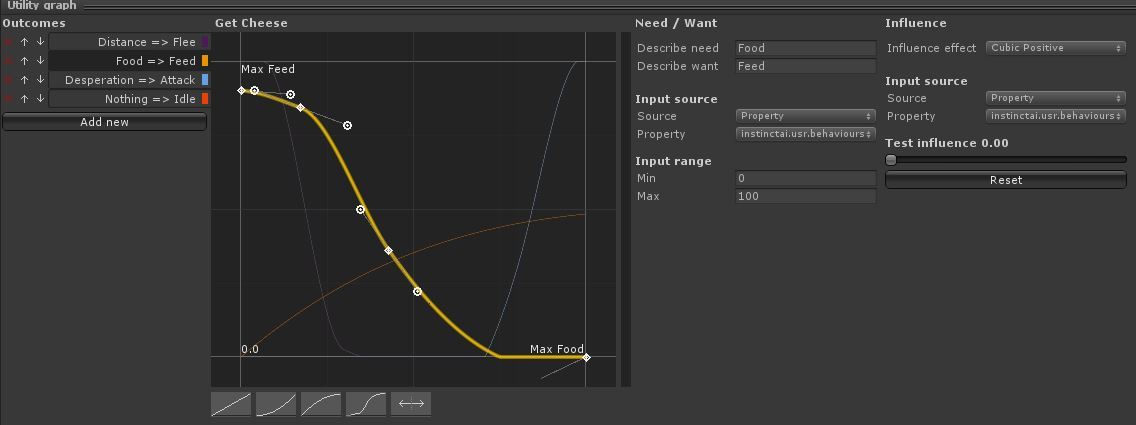
\includegraphics[width=0.9\textwidth]{instinctai}
    \end{center}
\end{frame}

\begin{frame}{Expected utility}
	\begin{itemize}
        \pause\item If the environment is \textbf{stochastic}, the outcome of an action (and hence its utility)
            may not be known with certainty
		\pause\item Let $p(x)$ be the probability that a given action has utility $x$
		\pause\item Then the \textbf{expected utility} is
            $$ \sum_x x \cdot p(x) $$
        \pause\item That is, the sum of utility values weighted by their probabilities
	\end{itemize}
\end{frame}

\begin{frame}{Expected utility --- example}
	\begin{itemize}
		\pause\item A slot machine pays out:
			\begin{itemize}
				\pause\item $\pounds 1$ with probability $0.05$
				\pause\item $\pounds 5$ with probability $0.03$
				\pause\item $\pounds 10$ with probability $0.02$
				\pause\item Nothing with probability $0.9$
			\end{itemize}
		\pause\item The expected payout is
			$$ 1 \times 0.05 + 5 \times 0.03 + 10 \times 0.02 + 0 \times 0.9
				= 0.4 $$
			i.e.\ $\pounds 0.40$
        \pause\item If it costs $\pounds 1$ to play the slot machine, the expected utility overall is
            $-\pounds 0.60$
        \pause\item (Although the actual utility can range from $-\pounds 1$ to $+\pounds 9$)
	\end{itemize}
\end{frame}

\begin{frame}{Inertia}
    \begin{itemize}
        \pause\item Utilities will generally change rapidly as the state of the environment changes
        \pause\item This could result in the agent \textbf{changing its mind} as to which action has the best utility
        \pause\item Can force the agent to finish its current action before evaluating and choosing another
        \pause\item Can give a utility bonus to sticking to the current action ---
            this still allows the agent to change its mind if the current action's utility becomes very bad
	\end{itemize}
\end{frame}

\begin{frame}{Multi-objective optimisation}
    \begin{itemize}
        \pause\item Utility-based AI is \textbf{single-objective}:
            all decision factors must be combined into a single number
        \pause\item An alternative is \textbf{multi-objective}:
            treat all decision factors as separate, and find an action that optimises all of them at once
    \end{itemize}
\end{frame}

\begin{frame}{Pareto optimality}
    \begin{columns}
        \begin{column}{0.5\textwidth}
            \begin{itemize}
                \pause\item Consider the space of all possible solutions (e.g.\ actions or plans)
                \pause\item A solution is \textbf{Pareto dominated} if there is some other solution
                    that is better than it on \textbf{all} decision factors at once
                \pause\item A solution is \textbf{Pareto optimal} if it is not dominated by any other solution
            \end{itemize}
        \end{column}
        \begin{column}{0.45\textwidth}
            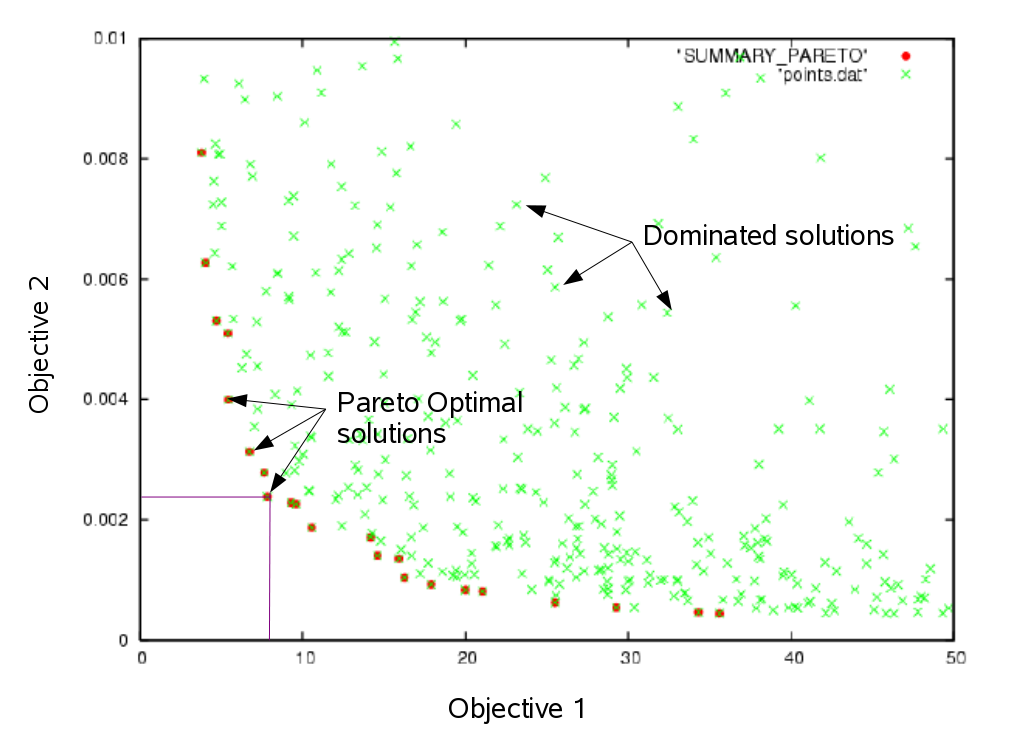
\includegraphics[width=\textwidth]{pareto}
        \end{column}
    \end{columns}
\end{frame}

\begin{frame}{Single-objective vs multi-objective}
    \begin{itemize}
        \pause\item Multi-objective optimisation gets around the problem of having to tune weights for
            decision factors
        \pause\item However, there are generally a large number of Pareto optimal solutions so we need some
            other method to tie-break between them
    \end{itemize}
\end{frame}



\end{document}
